\newtheorem{theorem}{Teorema}[section]  % se ha reinicializado con la sección, si no se numeraría con ordinales continuos
\newtheorem{example}[theorem]{Exercício}
\newtheorem{definition}[theorem]{Definição}

\newcommand{\bom}{
\begin{tikzpicture}[line width=2pt,scale=0.2]
\draw (-1,0) .. controls (-2.5,3.5) and (2.5,3.5) .. (1,0);
\draw (-1,0) .. controls (0,-0.2) .. (1,0);
\draw (-1,0)--(-0.9,-0.2);\draw (1,0)--(0.9,-0.2);
\shade[shading=ball, ball color=yellow] (-1,0) .. controls (-2.5,3.5) and (2.5,3.5) .. (1,0);
\shade[shading=ball, ball color=yellow] (-1,0) .. controls (0,-0.2) .. (1,0);
\shade[shading=ball, ball color=yellow] (-1,0)--(-0.9,-0.2);\draw (1,0)--(0.9,-0.2);
\fill[color=gray] (-0.9,-0.2) .. controls (0,-0.4) .. (0.9,-0.2);
\draw (-0.9,-0.2)--(-0.8,-0.4);\draw (0.9,-0.2)--(0.8,-0.4);
\fill[color=gray] (-0.8,-0.4) .. controls (0,-0.6) .. (0.8,-0.4);
\draw (-0.8,-0.4)--(-0.7,-0.6);\draw (0.8,-0.4)--(0.7,-0.6);
\fill[color=gray] (-0.7,-0.6) .. controls (0,-0.8) .. (0.7,-0.6);
\draw (-0.7,-0.6)--(-0.5,-0.8);\draw (0.7,-0.6)--(0.5,-0.8);
\fill[color=black] (-0.5,-0.8) .. controls (0,-1) .. (0.5,-0.8);
\draw (-0.5,-0.8) .. controls (0,-1) .. (0.5,-0.8);
\draw (-0.3,-0.15)..controls (0,1.3) .. (-0.5,1.5);
\draw (0.3,-0.15)..controls (0,1.3) .. (0.5,1.5);
\draw (0.5,1.5)..controls (0,1.3) .. (-0.5,1.5);
\end{tikzpicture}}
\newcommand{\bomapa}{
\begin{tikzpicture}[line width=2pt,scale=0.2]
\draw (-1,0) .. controls (-2.5,3.5) and (2.5,3.5) .. (1,0);
\draw (-1,0) .. controls (0,-0.2) .. (1,0);
\draw (-1,0)--(-0.9,-0.2);\draw (1,0)--(0.9,-0.2);
\shade[shading=ball, ball color=gray] (-1,0) .. controls (-2.5,3.5) and (2.5,3.5) .. (1,0);
\shade[shading=ball, ball color=gray] (-1,0) .. controls (0,-0.2) .. (1,0);
\shade[shading=ball, ball color=gray] (-1,0)--(-0.9,-0.2);\draw (1,0)--(0.9,-0.2);
\fill[color=gray] (-0.9,-0.2) .. controls (0,-0.4) .. (0.9,-0.2);
\draw (-0.9,-0.2)--(-0.8,-0.4);\draw (0.9,-0.2)--(0.8,-0.4);
\fill[color=gray] (-0.8,-0.4) .. controls (0,-0.6) .. (0.8,-0.4);
\draw (-0.8,-0.4)--(-0.7,-0.6);\draw (0.8,-0.4)--(0.7,-0.6);
\fill[color=gray] (-0.7,-0.6) .. controls (0,-0.8) .. (0.7,-0.6);
\draw (-0.7,-0.6)--(-0.5,-0.8);\draw (0.7,-0.6)--(0.5,-0.8);
\fill[color=black] (-0.5,-0.8) .. controls (0,-1) .. (0.5,-0.8);
\draw (-0.5,-0.8) .. controls (0,-1) .. (0.5,-0.8);
\draw (-0.3,-0.15)..controls (0,1.3) .. (-0.5,1.5);
\draw (0.3,-0.15)..controls (0,1.3) .. (0.5,1.5);
\draw (0.5,1.5)..controls (0,1.3) .. (-0.5,1.5);
\end{tikzpicture}}



\section*{Introdução}
O algoritmo Advanced Encryption Standard, abreviado com as siglas AES, é o algoritmo mais popular usado para proteção eletrónica de dados. Desde 2006, é o algoritmo mais popular dentro dos algoritmos usados no que se chama \emph{criptografia simétrica}. A criptografia simétrica também é denominada criptografia de um código, e é que o código que se usa tanto para cifrar uma mensagem como para a decifrar é o mesmo. Portanto, recetor e emissor concordam neste mesme código.

Com este artigo, pretende-se dar um esquema sobre como funciona este tipo de algoritmos, qual a matemática que o suporta, e formar uma ideia de que é o que acontece, por exemplo, quando passamos um cartão de pré-pagamento para o pagamento do bilhete do autocarro, ou como funcionam internamente os cartões pré-pagamento de energia como os que explicamos na Secção de Novidades deste número.

Em termos muito genéricos, temos um emissor e um recetor. O emissor dá uma informação (\textbf{input}) que é encriptada pelo algoritmo que apresentamos, o recetor recebe esta informação encriptada (\textbf{output}), e junto com o código secreto (\textbf{pin}) que é conhecido por ambos realiza o processo de desencriptação. Deste modo, foi transferida uma informação com alta segurança de que terceiros não possam ter acesso a ela. Veremos como é processada essa informação no algoritmo, como processa o código e como realiza o processo de encriptação, e em que tipo de matemática está suportado todo este jogo de encriptação. O processo de desencriptação não o veremos por ser bastante similar, mas a trabalhar de forma inversa.

\section{Bytes e vetor de bytes}
A unidade básica para processar no algoritmo AES é um {\textbf byte}: isso é uma sequência de oito bits tratado como uma unidade inteira. Um bit é um dígito do sistema binário. No sistema decimal, que é o que usualmente se usa na vida quotidiana, usamos 10 dígitos. No entanto, para o sistema binário apenas se necessitam dois dígitos, 0 e 1. A nível de placa informática, podemos imaginar o zero como desligado e o 1 como ligado. Ver um exemplo de um byte de oito bits representado na Figura \ref{fig:byte}.

\begin{figure}[!ht]
\begin{figurebox}
\begin{center}
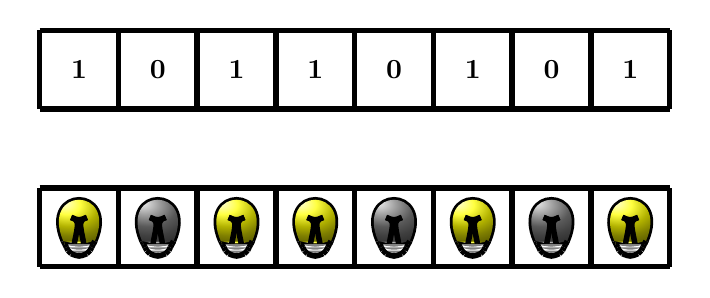
\begin{tikzpicture}[thick,line width=2pt]
\draw[step=1] (0,0) grid (8,1);
\node at (0.5,0.575) {\bom};
\node at (1.5,0.575) {\bomapa};
\node at (2.5,0.575) {\bom};
\node at (3.5,0.575) {\bom};
\node at (4.5,0.575) {\bomapa};
\node at (5.5,0.575) {\bom};
\node at (6.5,0.575) {\bomapa};
\node at (7.5,0.575) {\bom};
\draw[step=1] (0,2) grid (8,3);
\node at (0.5,2.5) {{\bf 1}};
\node at (1.5,2.5) {{\bf 0}};
\node at (2.5,2.5) {{\bf 1}};
\node at (3.5,2.5) {{\bf 1}};
\node at (4.5,2.5) {{\bf 0}};
\node at (5.5,2.5) {{\bf 1}};
\node at (6.5,2.5) {{\bf 0}};
\node at (7.5,2.5) {{\bf 1}};
\end{tikzpicture}
\end{center}\caption{Exemplo de um byte de 8 bits em representação animada e binária}\label{fig:byte}
\end{figurebox}
\end{figure}


 A partir da unidade do byte podemos definir uma lista de bytes ou uma matriz de bytes como se mostra nas Definições \ref{def1} e \ref{def2}.
\begin{definition}\label{def1}
Uma lista de bytes é uma sequência finita de $n\in \mathbb{N}$ bytes que podemos denotar como se segue,
$$a_0 a_1 ...a_{n-1}$$
em que $a_{i}$ é um byte para $i \in \{0,1,...,n-1\}$.
\end{definition}

\begin{definition}\label{def2}
Uma matriz de bytes é um conjunto ordenado em filas e colunas cujos elementos são bytes. Mais particularmente, diremos que $A$ é uma matriz de $m$ filas e $n$ colunas e os sus elementos serão denotados como $a_{ij}$ para $i \in \{1,2,\dots, m\}$ e $j \in \{1,2,\dots, n\}$ sendo $a_{ij}$ um byte.
\end{definition}
Ver um exemplo de uma matriz quadrada de tamanho $4$ na Figura \ref{fig:matrizbytes}.

\begin{figure}
\begin{figurebox}
\begin{center}
$
\left[
\begin{array}{cccc}
a_{11} & a_{12} & a_{13} & a_{14}\\
a_{21} & a_{22} & a_{23} & a_{24}\\
a_{31} & a_{32} & a_{33} & a_{34}\\
a_{41} & a_{42} & a_{43} & a_{44}\\
\end{array}
\right]=\left[
\begin{array}{c|c|c|c}
10001001 & 11110000 & 10101010 & 10010011\\\hline
10011111 & 10010100 & 01001001 & 10111111\\\hline
00001001 & 01010101 & 10101011 & 10011001\\\hline
01011101 & 10010011 & 10110001 & 01011101\\
\end{array}
\right]
$
\end{center}\caption{Exemplo de uma matriz de bytes}\label{fig:matrizbytes}
\end{figurebox}
\end{figure}



\subsection{Entradas(input), saídas(output) e código secreto}\label{ss:input}

A entrada e a saída para o algoritmo AES consiste em um array de 16 bytes, isto perfaz um total de 128 bits. No processo interno do algoritmo, estes 128 bits serão operados como uma matriz de bytes de 4 por 4 como foi visto na Figura \ref{fig:matrizbytes}. Desta forma, o input ou entrada do algoritmo é representado como o seguinte array   $in_{0}in_{1}...\,in_{15}$ e o output ou saída como  $out_{0}out_{1}...\,out_{15}$, em que cada  $in_{i}$ e  $out_{i}$ é um byte para $i \in \{0,1,...,15\}$. Internamente, a entrada e todas as modificações, que denominamos {\textsl estados intermédios}, que produzirá o algoritmo serão trabalhados como matrizes de bytes de tamanho $4$ por $4$, como se pode ver na Figura Figura \ref{fig:inout}.

\begin{figure}[!ht]
\begin{figurebox}
\begin{center}
\tiny{$ \underbrace{in_{0}in_{1}...\,in_{15}}_{\text{entrada}} \rightarrow
\left[
\begin{array}{cccc}
in_{0} & in_{4} & in_{8} & in_{12}\\
in_{1} & in_{5} & in_{9} & in_{13}\\
in_{2} & in_{6} & in_{10} & in_{14}\\
in_{3} & in_{7} & in_{11} & in_{15}\\
\end{array}
\right] \rightarrow \underbrace{\left[
\begin{array}{cccc}
s_{00} & s_{01} & s_{02} & s_{03}\\
s_{10} & s_{11} & s_{12} & s_{13}\\
s_{20} & s_{21} & s_{22} & s_{23}\\
s_{30} & s_{31} & s_{32} & s_{33}\\
\end{array}
\right]}_{\text{estados intermedios}} \rightarrow \left[
\begin{array}{cccc}
out_{0} & out_{4} & out_{8} & out_{12}\\
out_{1} & out_{5} & out_{9} & out_{13}\\
out_{2} & out_{6} & out_{10} & out_{14}\\
out_{3} & out_{7} & out_{11} & out_{15}\\
\end{array}
\right] \rightarrow  \underbrace{out_{0}out_{1}...\,out_{15}}_{\text{salida}}
$
}
\end{center}\caption{Entrada, saída e estados intermédios.}\label{fig:inout}
\end{figurebox}
\end{figure}


No algoritmo os estados intermédios podem ver-se de outro ponto de vista. Os quatro bytes que formam cada coluna dão um total de 32 bits. Portanto, o estado pode ser interpretado como um vetor coluna de quatro palavras, cada uma delas formada com 32 bits. Assim, por exemplo, o estado intermédio representado na Figura \ref{fig:inout} pode ser considerado como um vetor coluna das seguintes palavras:
$$
w_0=s_{00}s_{10}s_{20}s_{30}, \quad w_1=s_{01}s_{11}s_{21}s_{31}, \quad, w_2=s_{02}s_{12}s_{22}s_{32}, \quad w_3=s_{03}s_{13}s_{23}s_{33}.
$$

O código secreto também é um array de bytes, mas temos três possibilidades: 16 bytes(128 bits), 24 bytes(192 bits) ou 32 bytes(256 bits). No caso de 128 bits, o código inicial e os posteriores processados no algoritmo serão processados como blocos de tamanho 4 por 4; no caso de 192 bits blocos de tamanho 4 por 6, e finalmente no caso de 256 bites blocos de tamanho 4 por 8.

\subsection{Interpretações diferentes de um byte}

Parece divertido que um byte de oito bits possa ser interpretado como um polinómio ou como um par de elementos hexadecimais. Vamos ver em que é que consiste isto. 

\begin{center}
\textbf{Notação polinomial}
\end{center}

Representamos um byte de oito dígitos como se segue $\{b_7, b_6,b_5,b_4,b_3,b_2,b_1,b_0\}$.  Este byte pode ser representado como um polinómio p(x) de grau sete como se segue:
\begin{equation}\label{eq:pol}
p(x)=b_7 x^7 +b_6 x^6+b_5 x^5+b_4 x^4+b_3 x^3+b_2 x^2+b_1 x+b_0=\sum_{k=0}^7 b_k x^k.
\end{equation}

Por exemplo, o byte $\{01101011\}$ representa o polinómio  $x^6+x^5+x^3+x+1$.

\begin{center}
\textbf{Notação hexadecimal}
\end{center}

O sistema hexadecimal consta de 16 dígitos:$0,1,2,3,4,5,6,7,8,9,A,B,C,D,E,F$. A letra $A$ representa 10, a letra $B$ onze, e assim sucessivamente. Por exemplo, o número 143 em notação decimal corresponde a $10011110$ em notação binária e a $9E$ com notação hexadecimal. A representação hexadecimal que vamos fazer de um byte é realizada mediante a seguinte representação:
\begin{center}
\begin{tabular}{|c|c||c|c||c|c||c|c|}\hline
Padrão & Caráter & Padrão & Caráter & Padrão & Caráter & Padrão & Caráter\\\hline
0000 & 0 & 0100 & 4 & 1000 & 8 & 1100 & C\\
0001 & 1 & 0101 & 5 & 1001 & 9 & 1101 & D\\
0010 & 2 & 0110 & 6 & 1010 & A & 1110 & E\\
0011 & 3 & 0111 & 7 & 1011 & B & 1111 & F\\\hline
\end{tabular}
\end{center}
Usando este padrão, se tomarmos, por exemplo, o byte  $\{10011110\}$	 corresponde em notação hexadecimal aos primeiros quatro dígitos corresponde a 9 em notação hexadecimal e os últimos quatro dígitos a E. Isto é, corresponde ao par 9E. Usando este padrão, podemos representar a matriz dada na Figura \ref{fig:matrizbytes} em notação hexadecimal como se segue:
$$\left[
\begin{array}{c|c|c|c}
89 & F0 & AA & 93\\\hline
9F & 94 & 49 & BF\\\hline
09 & 54 & AB & 99\\\hline
5D & 93 & B1 & 5D\\
\end{array}
\right].$$ 

\section{A matemática do algoritmo}
Todos os bytes no algoritmo AES são interpretados como polinómios de grau 7 com coeficientes  $0$ ou $1$. De um ponto de vista mais matemático e próprio, diríamos que os bytes estão interpretados como elementos do campo finito $\mathcal{GF}$($2^8$) (ver \cite{Hart}). Não vamos entrar em detalhes, e vamos falar da forma mais simples, mas se quiser saber mais do que é um corpo finito, os polinómios, as estruturas algebraicas, remeta-se às referências seguintes \cite{Hart,Hilton,HUnger}, é um mundo amazónico!

Vamos ver as operações que podemos fazer entre os bytes mediante a representação polinomial descrita na Equação (\ref{eq:pol}).
\subsection{Soma}\label{ss:suma}
Sejam dois bytes a $a=\{a_7,a_6,a_5,a_4,a_3,a_2,a_1,a_0\}$ e $b=\{b_7,b_6,b_5,b_4,b_3,b_2,b_1,b_0\}$, definimos a soma  $c=\{c_7,c_6,c_5,c_4,c_3,c_2,c_1,c_0\}$ entre $a$ e $b$ que denotamos como $a \oplus b$ que denotamos  como se segue:
\begin{description}
\item[Notação de byte:]
$c=a\oplus b=\{c_7,c_6,c_5,c_4,c_3,c_2,c_1,c_0\}=\{a_7 \oplus b_7,a_6 \oplus b_6,a_5 \oplus b_5,a_4 \oplus b_4,a_3 \oplus b_3,a_2 \oplus b_2,a_1\oplus b_1 ,a_0 \oplus b_0\}$ em que $\oplus$ denota a operação XOR binária, isto é: $0 \oplus 0=0, 1 \oplus 0=0 \oplus 1=1, 1 \oplus 1=0 $.
\item[Notação polinomial:] $\sum_{k=0}^7 c_k x^k=\sum_{k=0}^7 (a_k \oplus b_k) x^k$, sendo $\oplus$ a operação definida no anterior item.
\end{description}
\begin{example}
A soma do polinómio $x^7+x^6+x^4+x+1$ com $x^7+x^4+x+1$ dá $x^6$ como resultado o polinómio que corresponde ao byte $\{01000000\}$.
\end{example}

\subsection{Multiplicação}\label{ss:prod}
A multiplicação que vamos explicar não é tão intuitiva como a soma anterior. De facto, vamos abrir um intervalo para falar da operação {\sl módulo}.

La multiplicación que vamos a explicar no es tan intuitiva como la suma anterior. De hecho vamos a hacer una parada para hablar de la operación {\sl módulo}. 

Vamos reparar nisto: quando dividimos qualquer número natural por 2, temos duas opções de resto, 0 e 1. Esta distinção não é outra que falar de números pares e ímpares. Mais formalmente, sejam todos os números inteiros $\mathbb{Z}$ e realizemos a divisão entre dois. Temos uma coleção de números cujo resto é 0, e outros cujo resto é 1. Deste ponto de vista, podemos falar de $\mathbb{Z}_2$ (espaço cociente) que é um corpo com dois únicos elementos: a classe dos elementos pares e a classe dos elementos ímpares. Repare que a operação XOR binária definida antes tem muita relação com isto. De facto, entender a operação  $1 \oplus 1= 0$ é muito simples agora se pensar que {\sl a soma de dois números ímpares é um número par}.

Podemos pensar em fazer algo similar, por exemplo dividindo por 5. Desta forma, o conjunto de números inteiros poderia ser descomposto em 5 classes: os divisíveis por 5 (classe [0]), os que dão resto 1 (classe [1]), os que dão resto 2 (classe [2]) , os que dão resto 3 (classe [3]) e os que dão resto 4 (classe [4]). Em que classe se encontra o número 1234?

Acha a operação modular estranha? Imagina que podemos fazer o mesmo com polinómios? Pois, também se pode. Imaginemos o polinómio \mbox{$x^{13}+ x^{11}+x^9+x^8+ x^6+x^5+x^4+x^3+1$} e dividamo-lo pelo polinómio irredutível de grau oito: \mbox{$x^8+x^4+x^3+x+1$}. Se dividirmos ambos os polinómios (faça-o como exercício para recordar como dividir dois polinómios) o resto que fica é o polinómio: \mbox{$x^8+x^4+x^3+x+1$}. De forma mais genérica: se tivermos um polinómio $p(x)$ e um outro polinómio de menor ou igual grau $q(x)$, diremos que $r(x)$ é $p(x)$ módulo $q(x)$ sendo $r(x)$ o resto de dividir $p(x)$ entre $q(x)$.

Dado este suposto salto ou parêntese, vamos entender o porquê disto tudo. Como se intitula esta subsecção, a multiplicação, isto é multiplicação de dois polinómios que cada um deles representa um byte. Mas se recordar como multiplicar dois polinómios, o grau do polinómio produto é a soma dos graus dos polinómios. Por exemplo, se multiplicar um polinómio de grau 3 por outro de grau 6, o resultado será um polinómio de grau 9. Mas em todo o momento dissemos que o algoritmo AES trabalhará com polinómios de grau menor ou igual que 7. Então se multiplicarmos polinómios de grau, no máximo sete, teremos na maioria dos casos polinómios de grau maior que sete. Esta é a razão pela qual a multiplicação não é a usual, mas que a multiplicação que é definida é a usual seguida de uma operação modular com o polinómio irredutível seguinte:
\begin{equation}\label{eq:q}
q(x)=x^8+x^4+x^3+x+1.
\end{equation}
Ao ser $q(x)$ um polinómio de grau $8$, o resto terá sempre um grau no máximo $7$, obtendo o que queríamos, trabalhar com bytes. Esta multiplicação vamos denotá-la como $a(x) \bullet b(x)$ ou em notação de bytes como $a\bullet b$ entre $a$ e $b$.
\begin{example}
Sejam os polinómios $a(x)=x^6+x^4+x^2+x+1$ e $b(x)=x^7+x+1$, a sua multiplicação usual é \mbox{$x^{13}+ x^{11}+x^9+x^8+ x^6+x^5+x^4+x^3+1$} e operação modular com $q(x)$ dado na Equação (\ref{eq:q}) dá como resultado o polinómio \mbox{$x^7+x^6+1$}. Assim,
$$
a(x)\bullet b(x)=x^7+x^6+1.
$$
\end{example}
Observemos que na operação de multiplicar os polinómios se dá a multiplicação entre elementos binários, isto é: $1 \cdot 1=1, 1 \cdot 0= 0\cdot 1= 0, 0 \cdot 0 =0$.


%\subsection{Multiplicación por x}
%De nuevo, si tenemos un polinomio de a lo sumo grado siete si multiplicamos por $x$ este será a lo sumo de grado ocho, por lo que dejaríamos de %trabajar con polinomios de grado menor o igual que siete, es por ello que de nuevo hablamos de multiplicación realizando módulo el polinomio %$q(x)$ definido en la ecuación (\ref{eq:q}). Veamos que hacer esto da como resultado una operación curiosa. Veámoslo primero con unos ejemplos.

%Sea $z(x)=x^6+x^2+x+1$, entonces el polinomio $x \cdot z(x)= x^7+x^3+x^2+x$ y módulo $q(x)$ coincide con el mismo por ser de menor grado que %ocho. Tomemos otro ejemplo donde el coeficiente del monomio de grado 7 no es cero. Sea $s(x)=x^7+x^5+x^2+x+1$, entonces el polinomio $x \cdot %s(x)= x^8+x^6+x^3+x^2+x$ y si realicemos la división con el polinomio $q(x)$ dado en la Ecuación (\ref{eq:q}) tenemos que el resto es el %polinomio resultanter de realizar la operación $x \cdot s(x)-q(x)$. De esta maenra el resultado final es el polinomio $x^6+x^4+x^2+1$. Si %miramos esto con bytes, la operación de multiplicar por $x$ cuando $b_7 \neq 0$ (mire la notación expuesta en la ecuación (\ref{eq:pol})) es %equivalente ha crear un byte corriendo los digitos a la izquierda y realizar la operación XOR con el byte $(1b)=\{00011011\}$. Así el polinomio  %$s(x)$ del ejemplo anterior que se corresponde con el byte $(A7)=\{10100111\}$, le hacemos un movimiento a la izquierda y nos da  $\{01001111\}$ %y sumamos con $(1b)=\{00011011\}$, obteniendo el byte $(\{01010100\}$ que se corresponde con $x^6+x^4+x^2+1$. Esta operación es la que el %algoritmo AES ha denominado {\sl xtime()}. La repetición de esta operación permite la multiplicación de potencias de $x$.

\subsection{Polinómios com coficientes que são bytes de oito dígitos}

Na subsecção \ref{ss:input} falamos de palavras como uns vetores colunas de 32 bits concatenados. Vamos ver como trabalhar com tudo isto e a matemática que modeliza isto. Antes falámos de polinómios de grau menor ou igual a sete com coeficientes em $\mathbb{Z}_2$, isto é 0 ou 1. Agora vamos é definir o seguinte polinómio.
\begin{equation}\label{def:polwo}
a(x)=a_3 x^3+a_2 x^2+ a_1 x + a_0,
\end{equation}
em que $a_3,a_2,a_1$ e $a_0$ são bytes de oito dígitos. Vamos ver como fizemos nas anteriores subsecções com este tipo de polinómios, como sejam as operações soma e multiplicação entre dois polinómios dados como a equação (\ref{def:polwo}).
\subsubsection{Soma}\label{ss:sumarara}
Esta é muito intuitiva, uma vez que é suficiente somar os bytes como vimos na subsecção \ref{ss:suma}. Desta forma, sejam $a(x)=a_3 x^3+a_2 x^2+ a_1 x + a_0$ e $b(x)=b_3 x^3+b_2 x^2+ b_1 x + b_0$ dois polinómios como na equação  (\ref{def:polwo}), então a soma denotada como será a seguinte:
$$
a(x)+b(x)=(a_3 \oplus b_3) x^3+(a_2 \oplus b_2) x^2+ (a_1 \oplus b_1) x + (a_0 \oplus b_0).
$$
\begin{example}
Seja $a(x)=\{10000001\} x^3+\{11100001\} x^2+ \{10101010\} x +\{01010100\}$ e $b(x)=\{10000001\} x^3+\{00000001\} x^2+ \{10101010\} x +\{00000000\}$ polinómios com coeficientes bytes, é fácil conferir que 
$$
a(x)+b(x)=\{00000000\} x^3+\{11100000\} x^2+ \{00000000\} x +\{01010100\}.
$$
\end{example}
\subsubsection{Multiplicação}\label{ss:prodraro}
Esta operação segue um raciocínio similar ao realizado na subsecção \ref{ss:prod}. Mas é um pouco mais complicado.
\begin{description}
\item[Passo multiplicativo] Criamos o polinómio produto $c(x)$ a partir de $a(x)$ e $b(x)$ dados como antes, como se segue:
$$
c(x)=c_6x^6+c_5x^5+c_4 x^4+c_3 x^3 +c_2 x^2 +c_1 x+c_0,
$$
em que
\begin{equation}\label{eq:progf}
\begin{array}{ll}
c_0= a_0 \bullet b_0, & c_1=a_1\bullet b_0 \oplus a_0 \bullet b_1,\\
c_2=a_2\bullet b_0 \oplus a_1 \bullet b_1 \oplus a_0 \bullet b_2 , & c_3= a_3\bullet b_0 \oplus a_2 \bullet b_1 \oplus a_1 \bullet b_2 \oplus a_0\bullet b_3,\\
c_4=a_3\bullet b_1 \oplus a_2 \bullet b_2 \oplus a_1 \bullet b_3, &  c_5=a_3\bullet b_2 \oplus a_2 \bullet b_3,\\
c_6=a_3\bullet b_3. & \\   
\end{array}
\end{equation}
\item[Passo modular] Como o resultado na equação (\ref{eq:progf}) não é um polinómio de quatro palavras, temos que realizar uma operação modular com um polinómio de grau 4. O algoritmo AES realiza-o com o polinómio $x^4+1$. Esta operação vamos deixá-la como exercício para que pratique (pode ver todos os detalhes em \cite{Federal}).
\end{description}

Finalmente, se trabalhar o que propusemos, pode ver-se que realizar o produto entre  $a(x)$ e $b(x)$, o qual denotaremos como $a(x)\otimes b(x)$ , é equivalente a realizar uma operação matricial em que as somas e produtos são os explicados na subsecção anterior, isto é $\bullet$ e $\oplus$  entre bytes. Assim, \mbox{$a(x)\otimes b(x)=d(x)=d_3x^3+d_2 x^2+d_1 x+d_0$} em que
$$
\left[
\begin{array}{c}
d_0\\
d_1\\
d_2\\
d_3\\
\end{array}
\right]=\left[
\begin{array}{cccc}
a_0 & a_3 & a_2 & a_1\\
a_1 & a_0 & a_3 & a_2\\
a_2 & a_1 & a_0 & a_3\\
a_3 & a_2 & a_1 & a_2\\
\end{array}
\right]\left[
\begin{array}{c}
b_0\\
b_1\\
b_2\\
b_3\\
\end{array}
\right]
$$
Observemos que se tomamos como polinómio $a(x)=\{00000001\}x^3$ o resultado do produto de $a(x)\otimes b(x)$ é uma rotação da palavra $[b_0, b_1,b_2,b_3]$; isto é  $[b_1, b_2,b_3,b_0]$. Esta operação vai denotar o algoritmo AES como  {\textsl rotWord()}.
\section{Um esquema do algoritmo}
Antes de dar as ideias do algoritmo, queremos salientar vários pontos:
\begin{itemize}
\item A longitude da entrada e saída é de 128 bits representados em blocos de tamanho quatro por quatro, cada elemento um byte (usando notação hexadecimal será mais fácil representá-lo).
\item A longitude do código secreto dependerá do tipo de algoritmo AES que use. Distinguem-se três AES-128, AES-192 e AES-256, os quais usam um código secreto, respetivamente de 128 bits, 192 bits e 256 bits.
\item O número de voltas que se dará ao algoritmo dependerá também do tipo de AES. O AES.128 realizará 10 voltas, o AES-192 doze e o AES-256 realizará 14.
\end{itemize} 

Para não complicar demais o algoritmo, apenas veremos o processo de encriptação. O processo de desencriptação é similar mas com operações inversas.
\subsection{Input del algoritmo}
O estado e o código secreto. Usando notação hexadecimal teríamos algo assim
\begin{figure}[!ht]
\begin{figurebox}
\begin{center}
$\begin{array}{|c|c|c|c|}
\multicolumn{4}{c}{\text{ESTADO INICIAL}}\\\hline
04 & E0 & 48 & 28\\\hline
66 & CB & F8 & 06\\\hline
81 & 19 & D3 & 26\\\hline
E5 & 9A & 7A & 4C\\\hline
\end{array}
\quad
\begin{array}{|c|c|c|c|}
\multicolumn{4}{c}{\text{CODIGO SECRETA}}\\\hline
A0 & 88 & 23 & 2A\\\hline
FA & 54 & A3 & 6C\\\hline
FE & 2C & 39 & 76\\\hline
17 & B1 & 39 & 05\\\hline
\end{array}
$
\end{center}\caption{Input del Algoritmo AES-128}\label{fig:inputaes1}
\end{figurebox}
\end{figure}
\subsection{Processo de encriptação do estado}
Distinguimos três etapas:
\begin{center}{\bf Roda inicial}\end{center}
\begin{figure}[!ht]
\begin{figurebox}
\begin{center}
$\begin{array}{|c|c|c|c|}
\multicolumn{4}{c}{\text{ESTADO INICIAL}}\\\hline
04 & E0 & 48 & 28\\\hline
66 & CB & F8 & 06\\\hline
81 & 19 & D3 & 26\\\hline
E5 & 9A & 7A & 4C\\\hline
\end{array},
\begin{array}{|c|c|c|c|}
\multicolumn{4}{c}{\text{CÓDIGO SECRETO}}\\\hline
A0 & 88 & 23 & 2A\\\hline
FA & 54 & A3 & 6C\\\hline
FE & 2C & 39 & 76\\\hline
17 & B1 & 39 & 05\\\hline
\end{array}\rightarrow
\colorbox{pink}{AddRoundKey}\rightarrow \begin{array}{|c|c|c|c|}
\multicolumn{4}{c}{\text{ESTADO 0}}\\\hline
A4 & G8 & 6B & 02\\\hline
9C & 9F & 5B & 6A\\\hline
7F & 35 & EA & 50\\\hline
F2 & 2B & 43 & 49\\\hline
\end{array}
$
\end{center}\caption{Roda Inicial do algoritmo AES-128}\label{fig:inputaes1}
\end{figurebox}
\end{figure}


\begin{center}{\bf 9 rodas}\end{center}
\begin{figure}[!ht]
\begin{figurebox}
\begin{center}
$\begin{array}{|c|c|c|c|}
\multicolumn{4}{c}{\text{ESTADO $(i-1)$éSsimo}}\\\hline
A4 & G8 & 6B & 02\\\hline
9C & 9F & 5B & 6A\\\hline
7F & 35 & EA & 50\\\hline
F2 & 2B & 43 & 49\\\hline
\end{array}\rightarrow$
\begin{tabular}{l}
\\
\colorbox{green}{1. SubBytes}\\
\colorbox{yellow}{2. ShiftRows}\\
\colorbox{gray}{3. Mixcolums } \\
\colorbox{pink}{4. AddRoundKey} con 
\tiny{
$\begin{array}{|c|c|c|c|}
\multicolumn{4}{c}{\text{CLAVE $(i)$-éssima}}\\\hline
* & * & * & *\\\hline
* & * & * & *\\\hline
* & * & * & *\\\hline
* & * & * & *\\\hline
\end{array}$
}
\\
\end{tabular} $\rightarrow
\begin{array}{|c|c|c|c|}
\multicolumn{4}{c}{\text{ESTADO i+1-ésimo}}\\\hline
A4 & G8 & 6B & 02\\\hline
9C & 9F & 5B & 6A\\\hline
7F & 35 & EA & 50\\\hline
F2 & 2B & 43 & 49\\\hline
\end{array}
$
\end{center}\caption{Roda i-éssima do algoritmo AES-128 para $i\in\{1,2,...,9\}$}\label{fig:inputaes2}
\end{figurebox}
\end{figure}

\begin{center}{\bf Roda final}\end{center}
\begin{figure}[!ht]
\begin{figurebox}
\begin{center}
$\begin{array}{|c|c|c|c|}
\multicolumn{4}{c}{\text{ESTADO 9}}\\\hline
E9 & CB & 3D & AF\\\hline
09 & 31 & 32 & 2E\\\hline
89 & 07 & 7D & 2C\\\hline
72 & 5F & 94 & B5\\\hline
\end{array}\rightarrow$
\begin{tabular}{l}
\\
\colorbox{green}{1. SubBytes}\\
\colorbox{yellow}{2. ShiftRows}\\
\colorbox{pink}{3. AddRoundKey} con 
\tiny{
$\begin{array}{|c|c|c|c|}
\multicolumn{4}{c}{\text{CLAVE  9-ésima}}\\\hline
* & * & * & *\\\hline
* & * & * & *\\\hline
* & * & * & *\\\hline
* & * & * & *\\\hline
\end{array}$
}
\\
\end{tabular} $\rightarrow
\begin{array}{|c|c|c|c|}
\multicolumn{4}{c}{\text{ESTADO FINAL}}\\\hline
39 & 02 & DC & 19\\\hline
25 & DC & 11 & 6A\\\hline
84 & 09 & 85 & 0B\\\hline
1D & FB & 57 & 32\\\hline
\end{array}
$
\end{center}\caption{Última roda do algoritmo AES-128}\label{fig:inputaes3}
\end{figurebox}
\end{figure}

%\newpage

Nas Figuras \ref{fig:inputaes1}, \ref{fig:inputaes2} e \ref{fig:inputaes3} mostra-se um esquema do processo de encriptação do algoritmo AES e na. O processo de desencriptação é bastante análogo mas com operações inversas. Na secção em anexo vamos pôr claros exemplos do que fazem cada uma das operações que aparecem no esquema, estas são: SubBytes(), ShiftRows(), MixColumns(), AddRoundKey().

\subsection{Processo de código}
O código inicial irá modificando-se ao longo do processo para ser utilizado do modo que se apresenta nas figuras \ref{fig:inputaes2} e \ref{fig:inputaes3}. Este processo consiste em, dado o código inicial, o qual vamos ver como um array de quatro palavras, cada palavra serão os 32 bits que encontramos em cada coluna. Para gerar a primeira palavra do código ronda 1, o que se fará é aplicar à palavra 4 do atual código a operação {\sl RotWord()} que vimos na subsecção  \ref{ss:prodraro}, e depois de ter feito isto,  soma-se a primeira palavra e a primeira coluna da matriz Rcom que aparece na tabela \ref{tab:Rcon}. A segunda palavra é calculada a partir da calculada somando a segunda do código anterior; o mesmo com a terceira e a quarta. E este seria o código volta 1. As nove restantes são calculadas de forma análoga, utilizando sempre a anterior.

\begin{table}[ht!]
\begin{center}
$RCON=$\tiny{$\left[
\begin{array}{cccccccccc}
 01 & 02 & 04 & 08 & 10 & 20 & 40 & 80 & 1B & 36\\
 00 & 00 & 00 & 00 & 00 & 00 & 00 & 00 & 00 & 00\\
 00 & 00 & 00 & 00 & 00 & 00 & 00 & 00 & 00 & 00\\
 00 & 00 & 00 & 00 & 00 & 00 & 00 & 00 & 00 & 00\\
\end{array}\right]$}
\end{center}\caption{Matriz Rcon, cada coluna representa a potência $x^i$ modulo $q(x)$ para $i\in\{0,1,2,\dots, 9\}$.}\label{tab:Rcon}
\end{table}


\section{Conclusões}

O processo de desencriptação é muito similar ao mostrado, mas as operações que são utilizadas e que se explicam no Anexo 4 devem ser vistas de forma inversa. Todos os detalhes pode vê-los em 5. Se quiser ver exemplos, pode remeter-se a  \cite{Federal}, em que aparece um programa e códigos das partes dos algoritmos.

\newpage

\section*{Anexo: as operações do processo de encriptação}\label{Anexo}
Aqui vamos representar de maneira informal e com simples exemplos cada uma das operações que aparecem no processo de encriptação do Algoritmo RSA-128. Por simplicidade vamos trabalhar com notação hexadecimal.
\begin{enumerate}
\item {\bf SubBytes(\cdot)}: é uma transformação não linear que substitui cada byte de um estado por um outro utilizando uma tabela de substituição. Esta tabela é denominada S-box (ver \cite{Federal} ara ver a origem da mesma).
\begin{table}[ht!]
\begin{center}
\tiny{
\begin{tabular}{|c|c|c|c|c|c|c|c|c|c|c|c|c|c|c|c|c|c|}\hline
& & \multicolumn{16}{c|}{$y$}\\\hline
& &{\textbf 0} & {\textbf 1} & {\textbf 2} & {\textbf 3} & {\textbf 4} & {\textbf 5} & {\textbf 6} & {\textbf 7} & {\textbf 8} & {\textbf 9} & {\textbf A} & {\textbf B} & {\textbf C} & {\textbf D} & {\textbf E} & {\textbf F}\\
\multirow{16}{*}{$x$} & {\textbf 0} & 63 & 7C & 77 & 7B & F2 & 6B & 6F & C5 & 30 & 01 & 67 & 2B & FE & D7 & AB & 76 \\
                    & {\textbf 1} & CA & 82 & C9 & 7D & FA & 59 & 47 & F0 & AD & D4 & A2 & AF & 9C & A4 & 72 & C0 \\
                    & {\textbf 2} & B7 & FD & 93 & 26 & 36 & 3F & F7 & CC & 34 & A5 & E5 & F1 & 71 & D8 & 31 & 15 \\
                    & {\textbf 3} & 04 & C7 & 23 & C3 & 18 & 96 & 05 & 9A & 07 & 12 & 80 & E2 & EB & 27 & B2 & 75 \\
                    & {\textbf 4} & 09 & 83 & 2C & 1A & 1B & 6E & 5A & A0 & 52 & 3B & D6 & B3 & 29 & E3 & 2F & 84 \\
                    & {\textbf 5} & 53 & D1 & 00 & ED & 20 & FC & B1 & 5B & 6A & CB & BE & \textbf{39} & 4A & 4C & 58 & CF \\
                    & {\textbf 6} & D0 & EF & AA & FB & 43 & 4D & 33 & 85 & 45 & F9 & 02 & 7F & 50 & 3C & 9F & A8 \\
                    & {\textbf 7} & 51 & A3 & 40 & 8F & 92 & 9D & 38 & F5 & BC & B6 & DA & 21 & 10 & FF & F3 & D2 \\
                    & {\textbf 8} & CD & 0C & 13 & EC & 5F & 97 & 44 & 17 & C4 & A7 & 7E & 3D & 64 & 5D & 19 & 73 \\
                    & {\textbf 9} & 60 & 81 & 4F & DC & 22 & 2A & 90 & 88 & 46 & EE & B8 & 14 & DE & 5E & 0B & DB \\
                    & {\textbf A} & E0 & 32 & 3A & 0A & 49 & 06 & 24 & 5C & C2 & D3 & AC & 62 & 91 & 95 & E4 & 79 \\
                    & {\textbf B} & E7 & C8 & 37 & 6D & 8D & D5 & 4E & A9 & 6C & 56 & F4 & EA & 65 & 7A & AE & 08 \\
                    & {\textbf C} & BA & 78 & 25 & 2E & 1C & A6 & B4 & C6 & E8 & DD & 74 & 1F & 4B & BD & 8B & 8A \\
                    & {\textbf D} & 70 & 3E & B5 & 66 & 48 & 03 & F6 & 0E & 61 & 35 & 57 & B9 & 86 & C1 & 1D & 9E \\
                    & {\textbf E} & E1 & F8 & 98 & 11 & 69 & D9 & 8E & 94 & 9B & 1E & 87 & E9 & CE & 55 & 28 & DF \\
                    & {\textbf F} & 8C & A1 & 89 & 0D & BF & E6 & 42 & 68 & 41 & 99 & 2D & OF & B0 & 54 & BB & 16 \\
                      \hline
\end{tabular}
}
\end{center}\caption{Substituição do byte xy (formato hexadecimal).}
\end{table}
Desta forma, se tivermos o estado seguinte, 
$$\tiny{
\begin{array}{|c|c|c|c|}
\hline
19 & 2F & 78 & 4A\\\hline
AA & 43 & 23 & 5B\\\hline
23 & 11 & 3B & 45\\\hline
F2 & 08 & 2B & 34\\\hline
\end{array},
}$$ vamos substituir cada elemento deste bloco por um outro resultante da S-box. Por exemplo, o elemento posicionado na fila 2 e coluna 4 é $5B$. Portanto, tomamos o elemento resultante da S-box da fila que corresponde ao elemento $5$ e a coluna $B$, este novo elemento é $39$. De forma análoga é fácil ver que:\\
$$SubBytes\left(\tiny{
\begin{array}{|c|c|c|c|}
\hline
19 & 2F & 78 & 4A\\\hline
AA & 43 & 23 & 5B\\\hline
23 & 11 & 3B & 45\\\hline
F2 & 08 & 2B & 34\\\hline
\end{array}
}
\right)=\tiny{
\begin{array}{|c|c|c|c|}
\hline
D4 & 15 & BC & D6\\\hline
AC & 1A & 26 & 39\\\hline
C3 & 82 & C2 & 6E\\\hline
89 & 30 & F1 & 18\\\hline
\end{array}
}$$. 


\item  {\bf ShiftRows(\cdot)}: é uma transformação que a fila i-éssima $i-1$ mudanças cíclicas, para $i=\{1,2,3,4\}$. Por exemplo, se  $\tiny{
\begin{array}{|c|c|c|c|}
\hline
23 & 11 & 3B & 45\\\hline
\end{array}
}$ é a fila três de um estado, realizam-se duas mudanças cíclicas, isto é  $\tiny{
\begin{array}{|c|c|c|c|}
\hline
3B & 45 & 23 & 11\\\hline
\end{array}
}$. Desta forma podemos ver:\\
$$ShiftRows\left(\tiny{
\begin{array}{|c|c|c|c|}
\hline
D4 & 15 & BC & D6\\\hline
{\textbf AC} & 1A & 26 & 39\\\hline
{\textbf C3} & {\textbf 82} & C2 & 6E\\\hline
{\textbf 89} & {\textbf 30} & {\textbf F1} & 18\\\hline
\end{array}
}\right)=\tiny{
\begin{array}{|c|c|c|c|}
\hline
D4 & 15 & BC & D6\\\hline
1A & 26 & 39 & {\textbf AC}\\\hline
C2 & 6E & {\textbf C3} & {\textbf 82}\\\hline
18 & {\textbf 89} & {\textbf 30} & {\textbf F1}\\\hline
\end{array}.
}$$
\item  {\textbf MixColumns(\cdot)}: é uma transformação que reflete a operação matemática vista na subsecção \ref{ss:prodraro}. Consideramos cada coluna de um estado como os coeficientes de um polinómio da forma como na Equação  (\ref{def:polwo}), e cada uma dela será multiplicado pelo polinómio fixo $a(x)=\{03\}x3+\{01\}x2+\{01\}x+\{02\}.$. Assim, a operação  {\textbf MixColumns()} realizada em cada coluna  $s(x)$de um estado é a operação $s(x) \otimes a(x)$ definida em  \ref{eq:progf}. Pode tentar confirmar o seguinte:
$$MixColumns\left(\tiny{
\begin{array}{|c|c|c|c|}
\hline
D4 & E0 & B8 & 1E\\\hline
BF & B4 & 41 & 27\\\hline
5D & 52 & 11 & 98\\\hline
30 & AE & F1 & C5\\\hline
\end{array}
}\right)=\tiny{
\begin{array}{|c|c|c|c|}
\hline
04 & E0 & 48 & 28\\\hline
66 & CB & F8 & 06\\\hline
81 & 19 & D3 & 26\\\hline
E5 & 9A & 7A & 4C\\\hline
\end{array}.
}$$
\item  {\textbf AddRoundkey(\cdot,\cdot)}: é uma transformação que tem dois argumentos, um estado e um código e a operação que se realiza é elemento a elemento a soma explicada na subsecção  \ref{ss:suma}. O seguinte exemplo mostra o seguinte:
$$MixColumns\left(\tiny{
\underbrace{\begin{array}{|c|c|c|c|}
\hline
04 & E0 & 48 & 28\\\hline
66 & CB & F8 & 06\\\hline
81 & 19 & D3 & 26\\\hline
E5 & 9A & 7A & 4C\\\hline
\end{array}}_{\text{estado}}
}, \tiny{
\underbrace{\begin{array}{|c|c|c|c|}
\hline
A4 & 88 & 23 & 2A\\\hline
9C & 54 & A3 & 6C\\\hline
7F & 2C & 39 & 76\\\hline
F2 & B1 & 39 & 05\\\hline
\end{array}}_{\text{código secreto}}
}\right)=\tiny{
\begin{array}{|c|c|c|c|}
\hline
A4 & 68 & 6B & 02\\\hline
9C & 9F & 5B & 6A\\\hline
7F & 35 & EA & 50\\\hline
F2 & 2B & 43 & 49\\\hline
\end{array}.
}$$

\end{enumerate}

\bibliographystyle{plain}
\bibliography{catenaria}

\newpage
%%% Local Variables: 
%%% mode: latex
%%% TeX-master: "matematicaseningenieria"
%%% End: 
